\documentclass[conference]{IEEEtran}
\IEEEoverridecommandlockouts
% The preceding line is only needed to identify funding in the first footnote. If that is unneeded, please comment it out.
\usepackage{cite}
\usepackage{amsmath,amssymb,amsfonts}
\usepackage{algorithmic}
\usepackage{graphicx}
\usepackage{textcomp}
\usepackage{xcolor}
\usepackage{appendix}
\usepackage{derivative}
\usepackage{tcolorbox}
\usepackage{subcaption}
\usepackage{lipsum}

\usepackage{cite}
\usepackage{amsmath,amssymb,amsfonts}
\usepackage{algorithmic}
\usepackage{graphicx}
\usepackage{textcomp}
\usepackage{xcolor}

 
\usepackage{minted}
\usepackage{tcolorbox}
\tcbuselibrary{minted}

\newtcblisting{mycodelisting}[1]{%
  listing engine=minted,
  minted style=default,
  minted language=python,
  minted options={fontsize=#1},
  listing only
}


\def\BibTeX{{\rm B\kern-.05em{\sc i\kern-.025em b}\kern-.08em
    T\kern-.1667em\lower.7ex\hbox{E}\kern-.125emX}}
    
\begin{document}


\title{AeroSense Explorer }

\author{\IEEEauthorblockN{Md. Tareq Monour\IEEEauthorrefmark{1}, Molla Md. Baki Billah \IEEEauthorrefmark{2}, Md. Asif Ahmed Tushar \IEEEauthorrefmark{3}, Mst. Sayma Akter \IEEEauthorrefmark{4} Md. Rahatul Islam \IEEEauthorrefmark{5}}
\IEEEauthorblockA{\textit{Dept. of Computer Science and Engineering} \\
\textit{United International University, Dhaka, Bangladesh}\\
011221519\IEEEauthorrefmark{1}, 011221197\IEEEauthorrefmark{2},
011221388\IEEEauthorrefmark{3}, 011221457\IEEEauthorrefmark{4} and 011221192\IEEEauthorrefmark{5}
}}

\maketitle

\begin{abstract}

The Aerospace Explorer remote-controlled (RC) aircraft that my team at United International University, MetaFive, has developed is called the AeroSense Explorer. This multi-sensor remote-controlled aircraft, outfitted with an array of sensors and parts, is a noteworthy progression in aerial technology. The AeroSense Explorer, built for intelligence and adaptability, can be used for a wide range of tasks, including light cargo transport, environmental monitoring, and recreational flying. Its extensive sensor suite allows it to identify changes in temperature, humidity, and obstacles in its path. Moreover, it can transmit real-time video data to a base station and carry and drop payloads. In the future, the team plans to implement fully autonomous operations to further enhance the capabilities of the AeroSense Explorer. Potential future developments could involve the integration of ground object detection systems and GPS navigation, thereby increasing their usefulness.
  Index Terms- IOT, Arduino, Sonar, GPS
\end{abstract}

\begin{IEEEkeywords}
IoT, Arduino, Sonar, GPS, Controller
\end{IEEEkeywords}


\section{Introduction}



The integration of fixed-wing drones into various applications poses several challenges that need to be addressed to fully realize their potential. This paper aims to identify and address key issues related to the design, operation, and utilization of fixed-wing drones, including but not limited to aerodynamic efficiency, autonomous navigation, payload capacity, and regulatory compliance. By elucidating these challenges and proposing potential solutions, this paper seeks to contribute to the advancement of fixed-wing drone technology and its widespread adoption across diverse domains.

Multiple fixed-wing unmanned aerial vehicles (UAVs) can be used to cooperatively track an uncooperative and moving target. A fixed-wing drone that uses a wing to provide lift, can fly at high altitudes, and has more endurance and range than all other types of drones. A single rotor has greater efficiency than a multi-rotor. The multirotor drone is commonly used for aerial photography, but it has limited endurance and speed\cite{hayat2020multi}. During the conceptual design stage, sketches start with an approximate sketch of the following: wing design, wing configuration, fuselage sizing, tail geometries, engine, and material selection. Fixed-wing drones are controlled by balancing aerodynamic forces and moments for stability and maneuverability. Other known fixed-wing drones can fly at about 4700 m above sea level, like the eBee drone\cite{mwenegoha2019enhanced}. Flying wings are mostly used for aerobatic flights; they perform loops, rolls, and other feats of spectacular flying performances.

Fixed-wing drones are entirely different in design and build from multi-rotor drones. They use a ‘wing’ like the normal airplanes out there. Unlike multi-rotor drones, fixed-wing type models never utilize energy to stay afloat in the air (fixed-wing types can’t stand still in the air) fighting gravity. Instead, they move forward on their set course or as set by the guide control (possibly a remote unit operated by a human) as long as their energy source permits. Most fixed-wing drones have an average flying time of a couple of hours. Gas-engine-powered drones can fly for up to 16 hours or more. It’s not easy to put a fixed-wing drone in the air. You either need a ‘runway’ or a catapult launcher to set a fixed-wing drone on course in the air. Flying a quadcopter doesn’t require special training. You just take them to an open area and fly them. Guiding and controlling a quadcopter can be learned on the go\cite{laupre2023reliable}.


\section{Project Overview}


In an era marked by rapid technological advancement and a growing need for efficient resource utilization, the development of autonomous systems has become increasingly crucial. Among these, fixed-wing drones represent a cutting-edge solution for various applications, offering unparalleled capabilities in aerial reconnaissance, mapping, surveillance, and beyond. The essence of the fixed-wing drone project lies in harnessing the power of unmanned aerial vehicles (UAVs) to perform a multitude of tasks traditionally carried out by manned aircraft or ground personnel\cite{grubesic2024overview}. By combining state-of-the-art aeronautical engineering with advanced automation and sensing technologies, the project aims to revolutionize the way we gather information, monitor landscapes, and execute missions in both civilian and military domains. At its core, the project entails the design, development, and implementation of a robust fixed-wing drone platform capable of autonomous flight operations. The system integrates sophisticated flight control algorithms, precision navigation systems, and real-time telemetry to enable seamless operation in diverse environments and scenarios. Key objectives of the project include:
\begin{enumerate}
    \item Designing a lightweight and aerodynamically optimized airframe to maximize flight endurance and range.
    \item Implementing intelligent flight control algorithms to ensure stable and precise maneuverability during autonomous missions.
    \item Integrating high-resolution imaging sensors, such as cameras and LiDAR, for comprehensive aerial data collection and analysis.
    \item Developing a user-friendly ground control station (GCS) interface for mission planning, monitoring, and post-flight analysis.
    \item Conducting rigorous testing and validation procedures to verify the performance, reliability, and safety of the drone system under various operating conditions.
    
\end{enumerate}
TDrones are classified according to their design configurations: rotor-wing, transitional, and fixed-wing drones\cite{HASSANALIAN201799}. Fixed-wing drones rely on their main wings for lift, while rotor-wing drones depend on propellers for both lift and forward motion. The motion of rotor-wing drones is controlled by speeding or slowing multiple downward thrusting motors.
Fixed-wing drone performance is affected by aerodynamic parameters and physical conditions such as wing design, altitude, wind forces, and payload distributions. One of the advantages of fixed-wing drones over rotor-wing drones is that they have better stability and control. They can be fitted with an autopilot to autonomously take off, fly longer distances, and land. They can be controlled to fly in a group by decentralized cooperative behavior, which implies that each drone in a group can act according to the mutual interests of the group. Through the deployment of fixed-wing drones, the project endeavors to enhance operational efficiency, reduce costs, and mitigate risks associated with conventional methods of aerial reconnaissance and surveillance\cite{cuniettiurban}. By leveraging the latest advancements in unmanned aerial technology, the project aims to pave the way for a future where autonomous drones play a central role in addressing critical challenges across industries and sectors.

\section{Component List}

Measures proportionately more than is customary. This measurement and others are deliberate, using specifications that anticipate your paper as one part of the entire proceedings, and not as an independent document. Please do not revise any of the current designations.

\begin{enumerate}
    \item Depron Board
    \item Arduino Uno
    \item NodeMcu ESP8266
    \item Electronic Speed Controllers (ESCs)
    \item Radio master controller
    \item Propellers
    \item LCD Display
    \item Battery
    \item Servo Motor(MG90S)
    \item Gas sensor(MQ135)
    \item DHT 11(Humidity Detection (Rain))
    \item Ultrasonic Sensor
    \item Carrier
    \item Jumper Wire
    \item Resistor
    \item Capacitor
    \item Breadboard
    \item Burner 
    \item Bluetooth module(HC06)
    \item Brushless motor (turnigy)
\end{enumerate}


\subsection{Depron Board}

Depron board, also known simply as Depron, is a brand name for a type of lightweight extruded polystyrene foam board. It's often used in hobbyist model-building, particularly in the construction of radio-controlled airplanes, drones, and architectural models.
\begin{figure}[th]
    \centering
    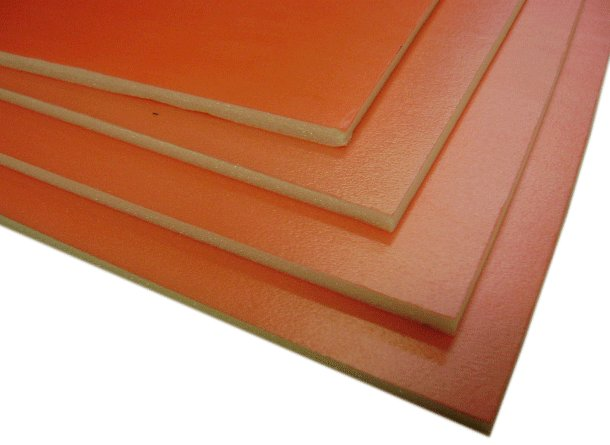
\includegraphics[width=\linewidth]{images/Depron Board.jpg}
    \caption{Depron Board}
    \label{fig:enter-label}
\end{figure}

Depron board is prized for its lightweight yet sturdy nature, making it ideal for creating model aircraft that can fly efficiently. It's easy to cut, shape, and glue, and it can be sanded to achieve smooth finishes. Its insulation properties also make it useful for other applications, such as insulation in buildings and even in artistic endeavors like sculpture-making.


\subsection{Arduino Uno}

Arduino is an open-source programmable circuit board that can be integrated into a wide variety of makerspace projects both simple and complex.  This board contains a microcontroller that can be programmed to sense and control objects in the physical world.   By responding to sensors and inputs, the Arduino can interact with a large array of outputs such as LEDs, motors, and displays.  Because of its flexibility and low cost, Arduino has become a very popular choice for makers and makerspaces looking to create interactive hardware projects.
\begin{figure}[th]
    \centering
    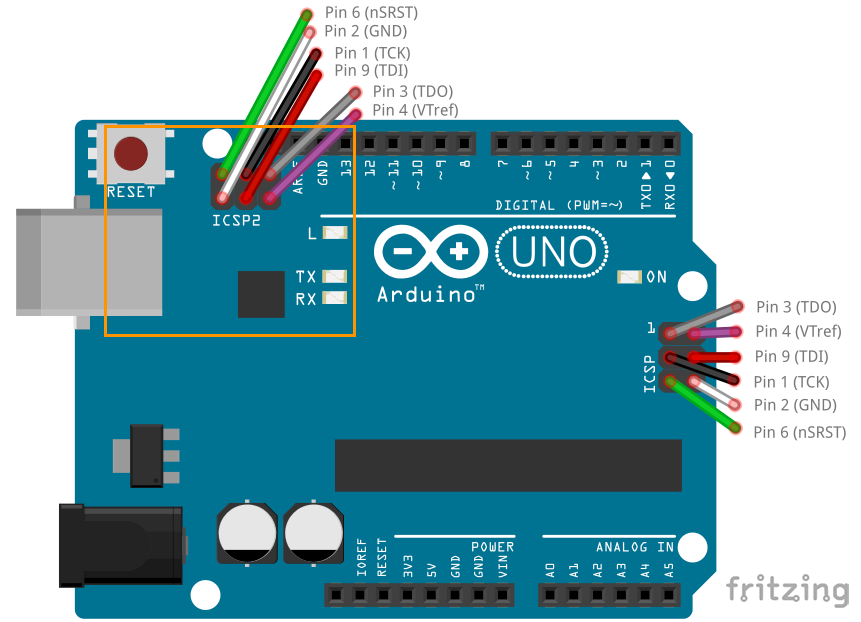
\includegraphics[width=\linewidth]{images/fritzing-arduino-uno-icsp.png}
    \caption{Arduino Uno}
    \label{fig:enter-label}
\end{figure}
The Arduino Uno is like a sturdy and flexible toolbox that many people in the DIY world use. It's a great starting point for learning about electronics and programming because it's open to everyone and has a big group of people who share ideas and help each other. This board is a simple and affordable way for anyone to start making cool things that can sense and control stuff in the real world. Whether you're just starting or you're already experienced, the Arduino Uno is there to support you and encourage you to explore new ideas and projects.

\subsection{NodeMcu ESP8266}

The NodeMCU ESP8266 is a popular development board based on the ESP8266 microcontroller chip. The ESP8266 is a low-cost Wi-Fi module that allows microcontrollers to connect to Wi-Fi networks and communicate with other devices or access the internet. The NodeMCU board integrates the ESP8266 chip with additional hardware components and provides a convenient platform for developing IoT (Internet of Things) projects and applications.
\begin{figure}[th]
    \centering
    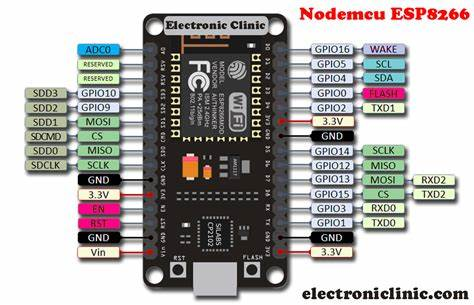
\includegraphics[height=4cm,width=\linewidth]{images/NODEMCU-ESP8266.jpg}
    \caption{NodeMcu ESP8266}
    \label{fig:enter-label}
\end{figure}

NodeMCU ESP8266 Specifications & Features:
\begin{enumerate}
    \item Microcontroller: Tensilica 32-bit RISC CPU Xtensa LX106
    \item Operating Voltage: 3.3V
    \item Input Voltage: 7-12V
    \item Digital I/O Pins (DIO): 16
    \item Analog Input Pins (ADC): 1
    \item UARTs: 1
    \item SPIs: 1
    \item I2Cs: 1
    \item Flash Memory: 4 MB
    \item SRAM: 64 KB
    \item Clock Speed: 80 MHz
    \item USB-TTL based on CP2102 is included onboard, Enabling Plug n Play
    \item PCB Antenna   
\end{enumerate}


So, it is an open-source Lua-based firmware and development board specially targeted for IoT-based Applications. It includes firmware that runs on the ESP8266 Wi-Fi SoC from Espressif Systems, and hardware that is based on the ESP-12 module.

\subsection{Electronic Speed Controllers (ESCs)}

 Fig.- HUBSAN ESC for H501S X4 FPV Quadcopter
Each motor has an ESC (though some designs put it all on one board). In its most basic form, an ESC regulates
power going to the motor with which it is paired. More sophisticated systems can also relay data back to
the MC, such as vitals about how the motors are performing. With six or more rotors, active feedback
makes it possible to keep flying (enough to land safely) if one motor fails.
\begin{figure}[th]
    \centering
    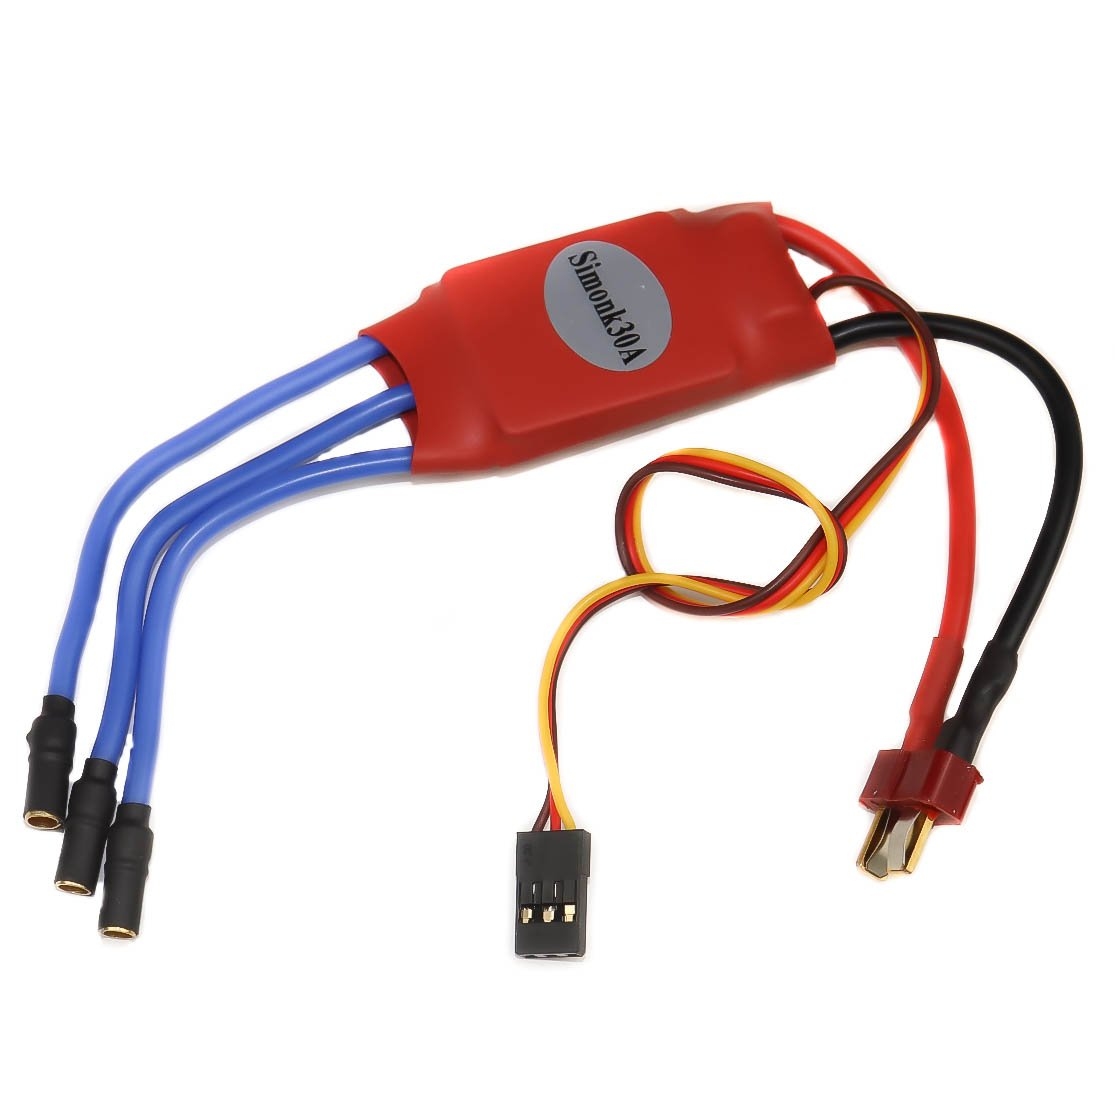
\includegraphics[height=5cm,width=\linewidth]{images/simonk 30 a.jpg}
    \caption{ESCs}
    \label{fig:enter-label}
\end{figure}

\subsection{Radio master controller}

The RadioMaster Pocket is a small, lightweight radio that packs a big punch. It is available in two versions, ExpressLRS and MPM CC2500, and both versions come preinstalled with EdgeTX firmware. The Pocket is also equipped with removable stick ends and a foldable antenna, making it easy to transport and store. It is compatible with 18650 batteries, which provide long battery life for hours of fun.
\begin{figure}[th]
    \centering
    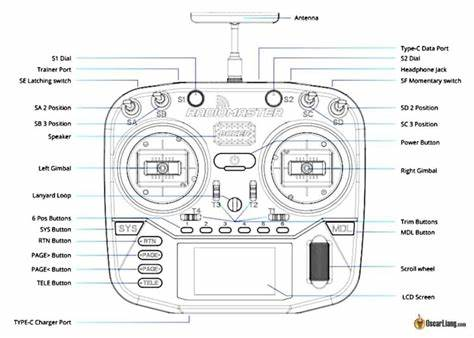
\includegraphics[height=5cm,width=\linewidth]{images/Radio master controller.jpg}
    \caption{Radio Master Controller}
    \label{fig:enter-label}
\end{figure}

\subsection{Propellers}

Fig.-veho Self-Tightening Propeller Blades for Muvi Drone
Light UAVs use plastic propellers, which resist breaking on impact because they are flexible, and they are
safer. Heavier models use carbon fiber or other more rigid materials (planes frequently use wood or
nylon/glass). Carbon fiber propellers are dangerous, even deadly, and should be used only by experienced
pilots and well away from people. Unless extreme performance is a concern, the benefits of carbon fiber over
plastic are marginal on multi-rotors.
Transmitter:
\begin{figure}[th]
    \centering
    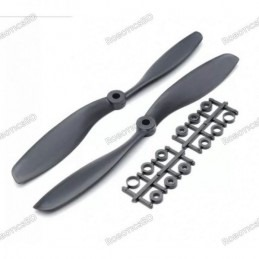
\includegraphics[width=\linewidth]{images/WhatsApp Image 2024-05-08 at 1.26.39 AM.jpeg}
    \caption{Propellers}
    \label{fig:enter-label}
\end{figure}
 Fig.3DR 2.4 GHz, 9-Channel Transmitter for IRIS Quadcopter
This is the radio controller. For an increasing number of tech toys and entry-level UAVs, the “transmitter” is
simply the combination of a mobile app and a Wi-Fi-enabled tablet or smartphone (Parrot uses Wi-Fi
control for all of its quadcopters). UAVs equipped with receivers, such as Spektrum and Futaba, can work
with a range of transmitters. This allows the user to select the best fit, depending on what features they are
looking for and what their budget might be. It should be noted: that these tend to be proprietary, so with a
Brand X receiver you'll probably need a Brand X or, at the very least, a Brand X-compatible transmitter.
Systems that include a transmitter (as well as other basic accessories required for flying) are dubbed
“ready-to-fly,” and are the simplest to jumpstart the beginner.
When investing in a transmitter, generally, compatibility can be determined by referring to the specs for
the receiver. It will need to support the same protocol as the receiver and support at least as many
channels as the receiver requires. So, for example, a DSMX 4-channel receiver will work happily with a
DSMX 6-channel transmitter. For advanced configurations, one also needs to consider secondary systems
that will need to inter-operate with the transmitter, such as a telemetry radio.
Transmitters can range anywhere from simple two-joystick jobs for remote-control toys to highly
sophisticated pieces of electronics with advanced programming to support myriad aircraft configurations,
expandable model memory, telemetry displays, audible feedback, and trainer ports. In many ways, higher transmitters are more complex than the aircraft they fly.
Other hardware systems that are not essential to the archetypical UAV but are nonetheless common,
include:
* GPS
* Optical flow
* Obstacle avoidance
* Telemetry/OSD
* Ground station

\subsection{LCD Display}

An I2C LCD, also known as a character LCD with an I2C interface, is a type of liquid crystal display module that communicates with a microcontroller using the I2C (Inter-Integrated Circuit) protocol. These displays are popular in Arduino and other microcontroller projects due to their ease of use and reduced pin requirement compared to traditional parallel interface LCDs.
\begin{figure}[h]
    \centering
    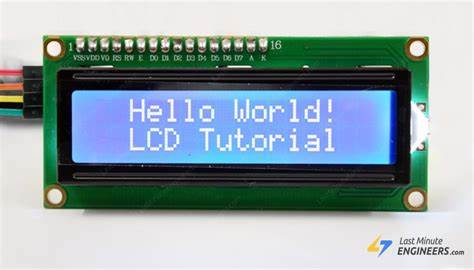
\includegraphics[width=\linewidth]{images/display.jpg}
    \caption{LCD Display}
    \label{fig:enter-label}
\end{figure}

\subsection{Battery}

In robotics or any project where power is a major concern, finding an alternative to lithium polymer batteries is a challenge. Lipo Battery 1100mAh 11.1V 3S Lithium polymer battery Pack (LiPo) battery is equipped with heavy-duty discharge leads to minimize resistance and sustain high current loads.
\begin{figure}[th]
    \centering
    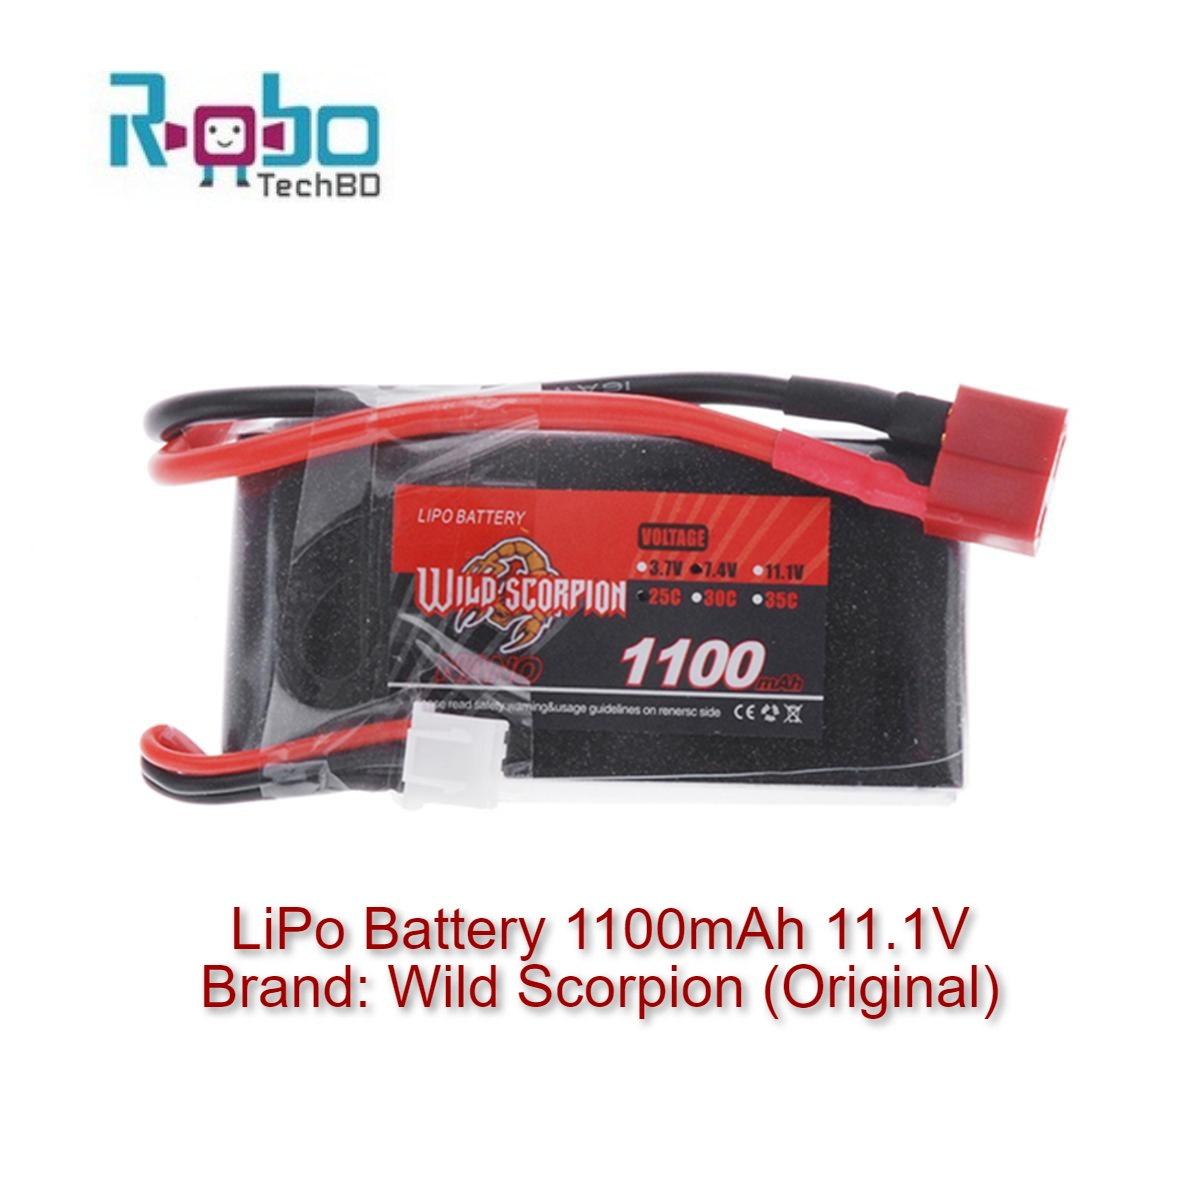
\includegraphics[height=4cm,width=\linewidth]{images/11.1V-Lipo-Battery-11mAh-1.jpg}
    \caption{Battery}
    \label{fig:enter-label}
\end{figure}
This Battery stands up to the punishing extremes of aerobatic flight and RC vehicles. Each pack is equipped with gold-plated connectors and JST-XH style balance connectors.


\subsection{Servo Motor(MG90S)}

MG90S is a micro servo motor with metal gear. This small and lightweight servo comes with high output power, thus ideal for  RC airplanes, quadcopters, or Robotic Arms.
\begin{figure}[th]
    \centering
    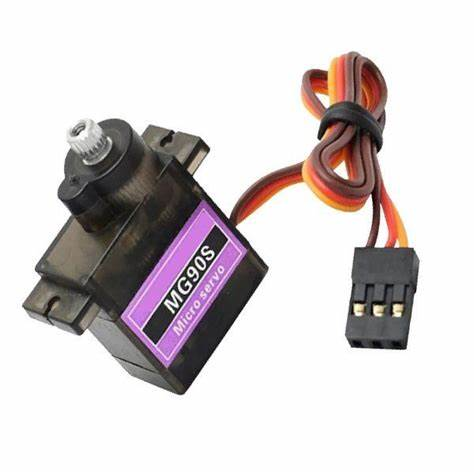
\includegraphics[height=5cm,width=\linewidth]{images/servo motor.jpg}
    \caption{Servo Motor}
    \label{fig:enter-label}
\end{figure}
MG-90S Features:
\begin{enumerate}
    \item Operating Voltage: 4.8V to 6V (Typically 5V)
    \item Stall Torque: 1.8 kg/cm (4.8V)
    \item Max Stall Torque: 2.2 kg/cm (6V)
    \item Operating speed is 0.1s/60° (4.8V)
    \item Gear Type: Metal
    \item Rotation: 0°-180°
    \item Weight of motor: 13.4gm
\end{enumerate}
The MG90S servo motor is a versatile and reliable component commonly used by hobbyists and makers due to its compact size, reasonable torque, and affordable price.


\subsection{Gas sensor(MQ-135)}

The MQ-135 Gas sensors are used in air quality control equipment and are suitable for detecting or measuring of NH3, NOx, Alcohol, Benzene, Smoke, and CO2. The MQ-135 sensor module comes with a Digital Pin which makes this sensor operate even without a microcontroller and that comes in handy when you are only trying to detect one particular gas. If we need to measure the gases in PPM, the analog pin needs to be used. The analog pin is TTL driven and works on 5V so can be used with most common microcontrollers.

MQ-135 Sensor Features:

\begin{enumerate}
    \item Wide detecting scope
    \item Fast response and High sensitivity
    \item Stable and long life
    \item Operating Voltage is +5V
    \item Detect/Measure NH3, NOx, alcohol, Benzene, smoke, CO2, etc.
    \item Analog output voltage: 0V to 5V
    \item Digital output voltage: 0V or 5V (TTL Logic)
    \item Preheat duration 20 seconds
    \item Can be used as a Digital or analog sensor
    \item The Sensitivity of the Digital pin can be varied using the potentiometer
    
\end{enumerate}
\begin{figure}[th]
    \centering
    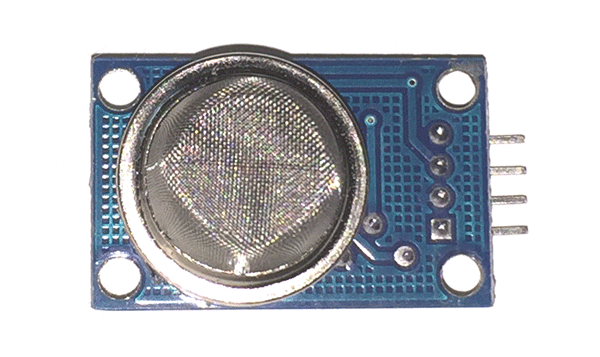
\includegraphics[height=5cm,width=\linewidth]{images/MQ-135-Sensor.png}
    \caption{MQ-135}
    \label{fig:enter-label}
\end{figure}

\subsection{Humidity Detection (Rain) DHT11}

The DHT11 is a basic, low-cost digital temperature and humidity sensor. It's capable of measuring both temperature and humidity levels in the surrounding environment. The DHT11 sensor utilizes a capacitive humidity sensor and a thermistor to measure the surrounding air, providing digital output for both temperature and humidity levels.
\begin{figure}[th]
    \centering
    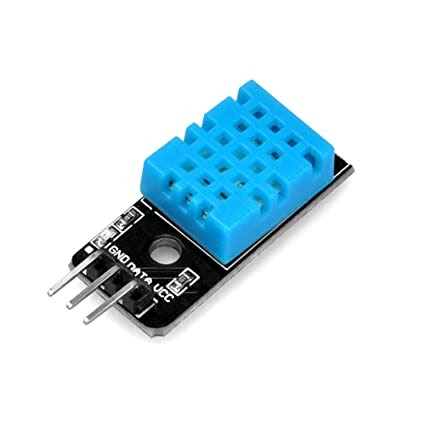
\includegraphics[height=5cm,width=\linewidth]{images/dh11.jpg}
    \caption{DHT-11}
    \label{fig:enter-label}
\end{figure}


\subsection{Ultrasonic Sensor (Obstacle Identify)}

An ultrasonic sensor is a device that measures the distance to an object by emitting ultrasonic sound waves and then measuring the time it takes for the waves to bounce back after hitting the object. The basic principle behind ultrasonic sensors involves emitting a burst of ultrasonic sound waves from a transducer, typically a piezoelectric crystal, and then detecting the reflected waves. By knowing the speed of sound in the air, the sensor can calculate the distance to the object based on the time it takes for the sound waves to travel to the object and back.
\begin{figure}[h]
    \centering
    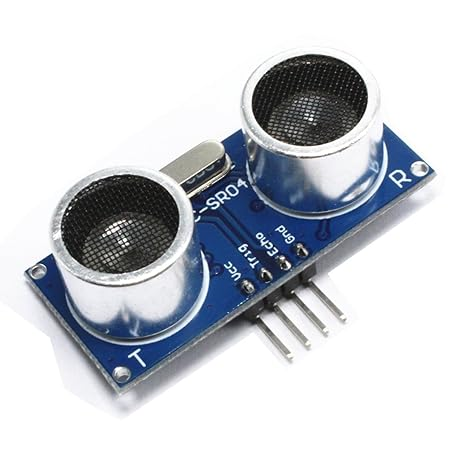
\includegraphics[height=4cm,width=\linewidth]{images/ultrasonic sensor.jpg}
    \caption{Ultrasonic Sensor}
    \label{fig:enter-label}
\end{figure}

\subsection{Jumper Wire}

Jumper wires are simple electrical wires used in electronics projects to create connections between different components on a breadboard or between various points on a circuit. They're typically made of flexible insulated wire, often with connectors at the ends such as pins or alligator clips to easily insert into breadboard holes or attach to components.
\begin{figure}[h]
    \centering
    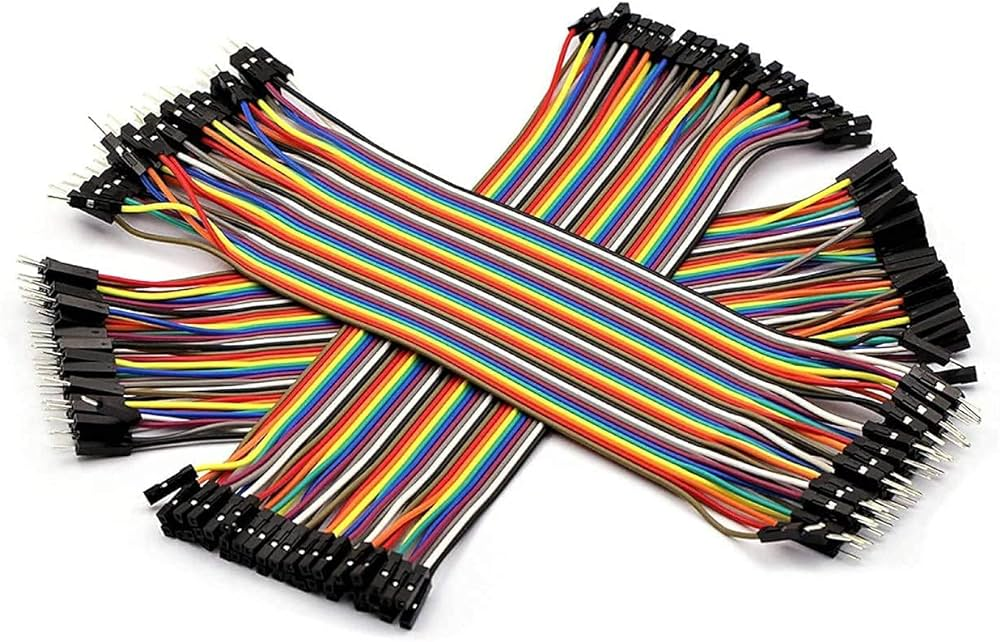
\includegraphics[height=3cm,width=\linewidth]{images/71zMG84YhsL._AC_UF1000,1000_QL80_.jpg}
    \caption{Jumper Wire}
    \label{fig:enter-label}
\end{figure}
We have used 3 types of Jumper wire. Those are - 
\begin{enumerate}
    \item Male to Male
    \item Male to Female
    \item Female to Female
\end{enumerate}

\subsection{Resistor}
\begin{figure}[h]
    \centering
    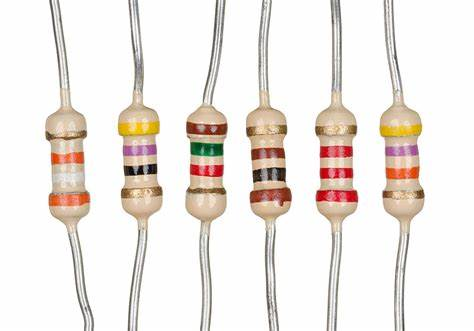
\includegraphics[height=3cm,width=\linewidth]{images/Resistor.jpg}
    \caption{Resistor}
    \label{fig:enter-label}
\end{figure}
A resistor is a passive two-terminal electrical component that implements electrical resistance as a circuit element. In electronic circuits, resistors are used to reduce current flow, adjust signal levels, divide voltages, bias active elements, and terminate transmission lines, among other uses. High-power resistors that can dissipate many watts of electrical power as heat may be used as part of motor controls, in power distribution systems, or as test loads for generators. Fixed resistors have resistances that only change slightly with temperature, time, or operating voltage. Variable resistors can be used to adjust circuit elements (such as a volume control or a lamp dimmer) or as sensing devices for heat, light, humidity, force, or chemical activity.


\subsection{Capacitor}

Capacitors are one of three fundamental electronic components that form the foundation of a circuit – along with resistors and inductors. A capacitor in an electrical circuit behaves as a charge storage device. It holds the electric charge when we apply a voltage across it, and it gives up the stored charge to the circuit when required.
\begin{figure}[th]
    \centering
    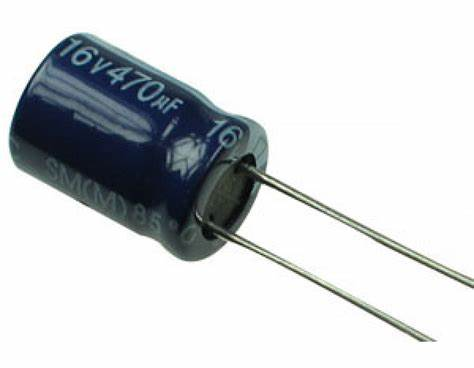
\includegraphics[height=4cm,width=\linewidth]{images/capasitor.jpg}
    \caption{Capasitor}
    \label{fig:enter-label}
\end{figure}

\subsection{Breadboard}

The breadboard is a circuit construction technique that is designed to allow the rapid creation of circuits without the need for soldering or making permanent connections. Leaded components (i.e. through-hole parts) are inserted into holes containing metal grips that gently clamp onto the lead and breadboards almost always have common rows whereby the holes in a row are electrically connected.
\begin{figure}[th]
    \centering
    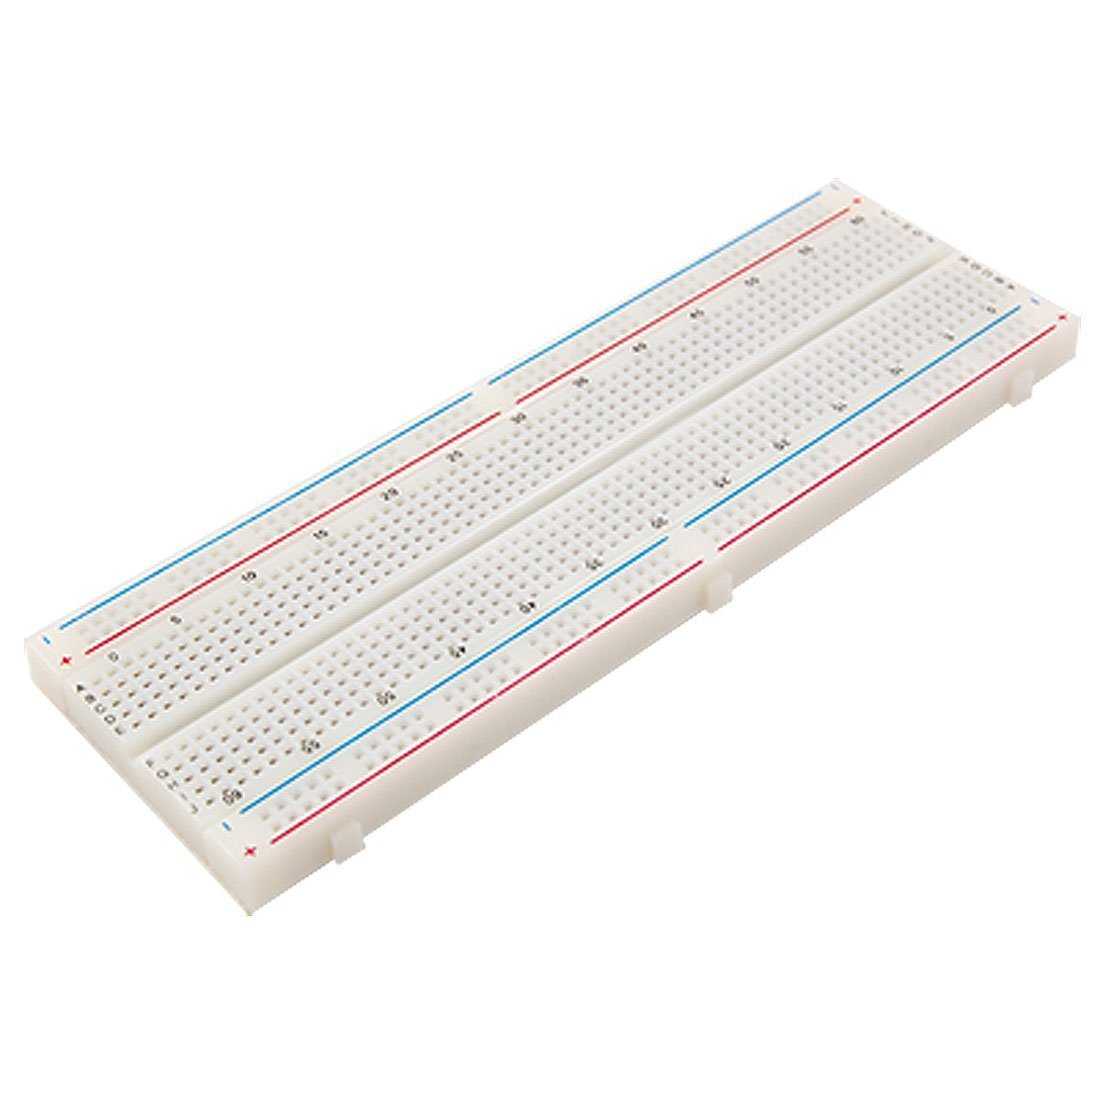
\includegraphics[height=5cm,width=\linewidth]{images/Breadboard.jpg}
    \caption{Breadboard}
    \label{fig:enter-label}
\end{figure}

\subsection{Burner}

This cable is commonly used to connect Arduino Uno, Arduino Mega 2560, Arduino 101, or any board with a USB female A port to your computer. It has a length of approximately 100 cm.
\begin{figure}[th]
    \centering
    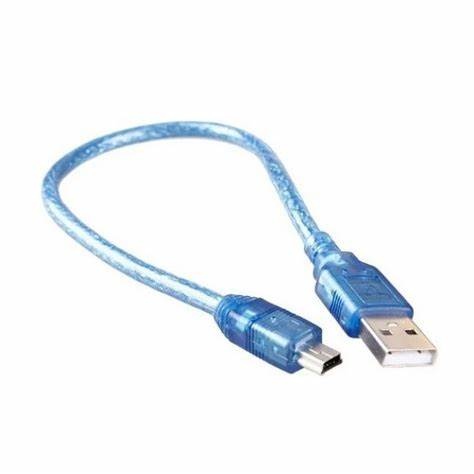
\includegraphics[height=4cm,width=\linewidth]{images/Burner Cable.jpg}
    \caption{Burner}
    \label{fig:enter-label}
\end{figure}

\subsection{Bluetooth module(HC06)}

HC-06 is a Bluetooth module designed for establishing short-range wireless data communication between two microcontrollers or systems. The module works on Bluetooth 2.0 communication protocol and it can only act as a slave device.
\begin{figure}[th]
    \centering
    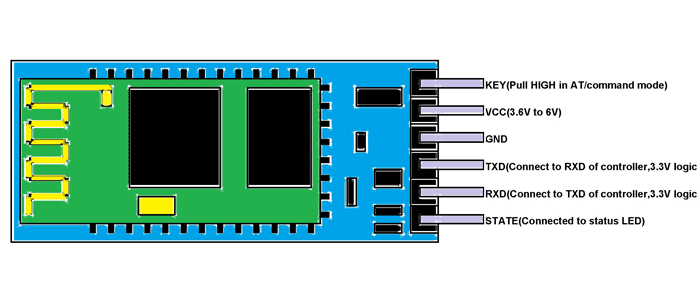
\includegraphics[width=\linewidth]{images/HC06-Bluetooth-module-pinout.png}
    \caption{HC06}
    \label{fig:enter-label}
\end{figure}

\subsection{Brushless motor (BLDC)}

\begin{figure}[th]
    \centering
    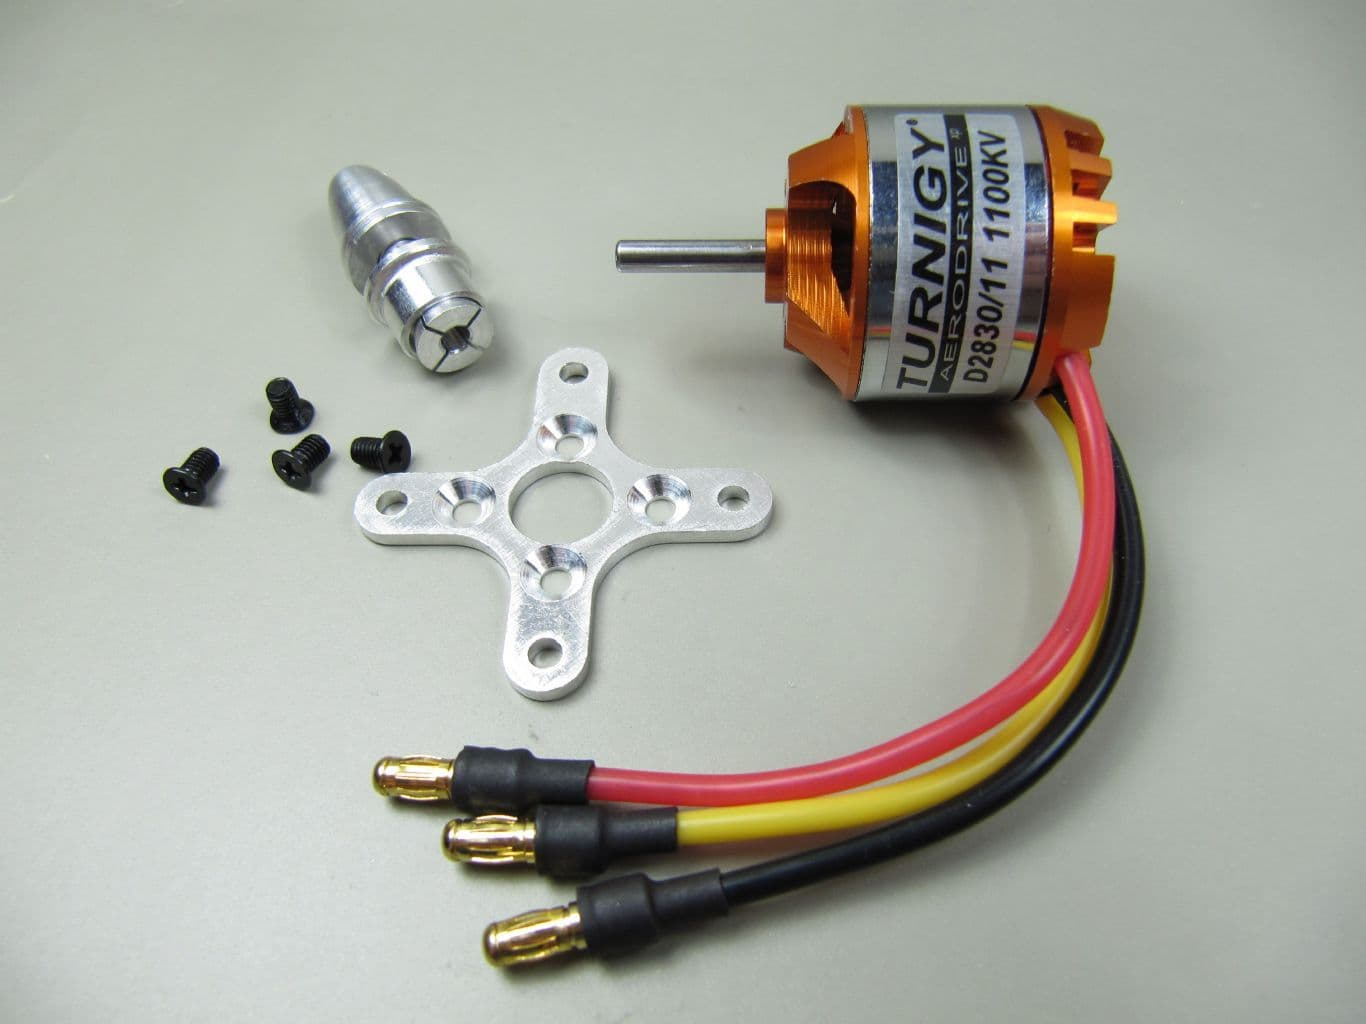
\includegraphics[height=5cm,width=\linewidth]{images/turnigy-d2830-11-1000kv-brushless-motor-v2-323-p.jpg}
    \caption{Brushless Motor}
    \label{fig:enter-label}
\end{figure}
Specs:
\begin{enumerate}
    \item Rpm/V: 1000kv
    \item Shaft: 3.17mm
    \item Voltage: 2S~4S (7.4v to 14.8v)
    \item Weight: 52g
    \item Watts: 210w
    \item Max Current: 21A
    \item ESC: 30A
    \item Suggested Prop: 8" to 10"
    \item Mounting Hole Bolt Circle: 16mm or 19mm
    
\end{enumerate}


\section{Implementation}

Implementing a feature on a fixed-wing drone involves several steps, but here's a brief overview\cite{ducard2009fault}\cite{mesquita2021steps}:
\begin{figure}[h]
    \begin{minipage}{0.47\textwidth}
        \flushright
        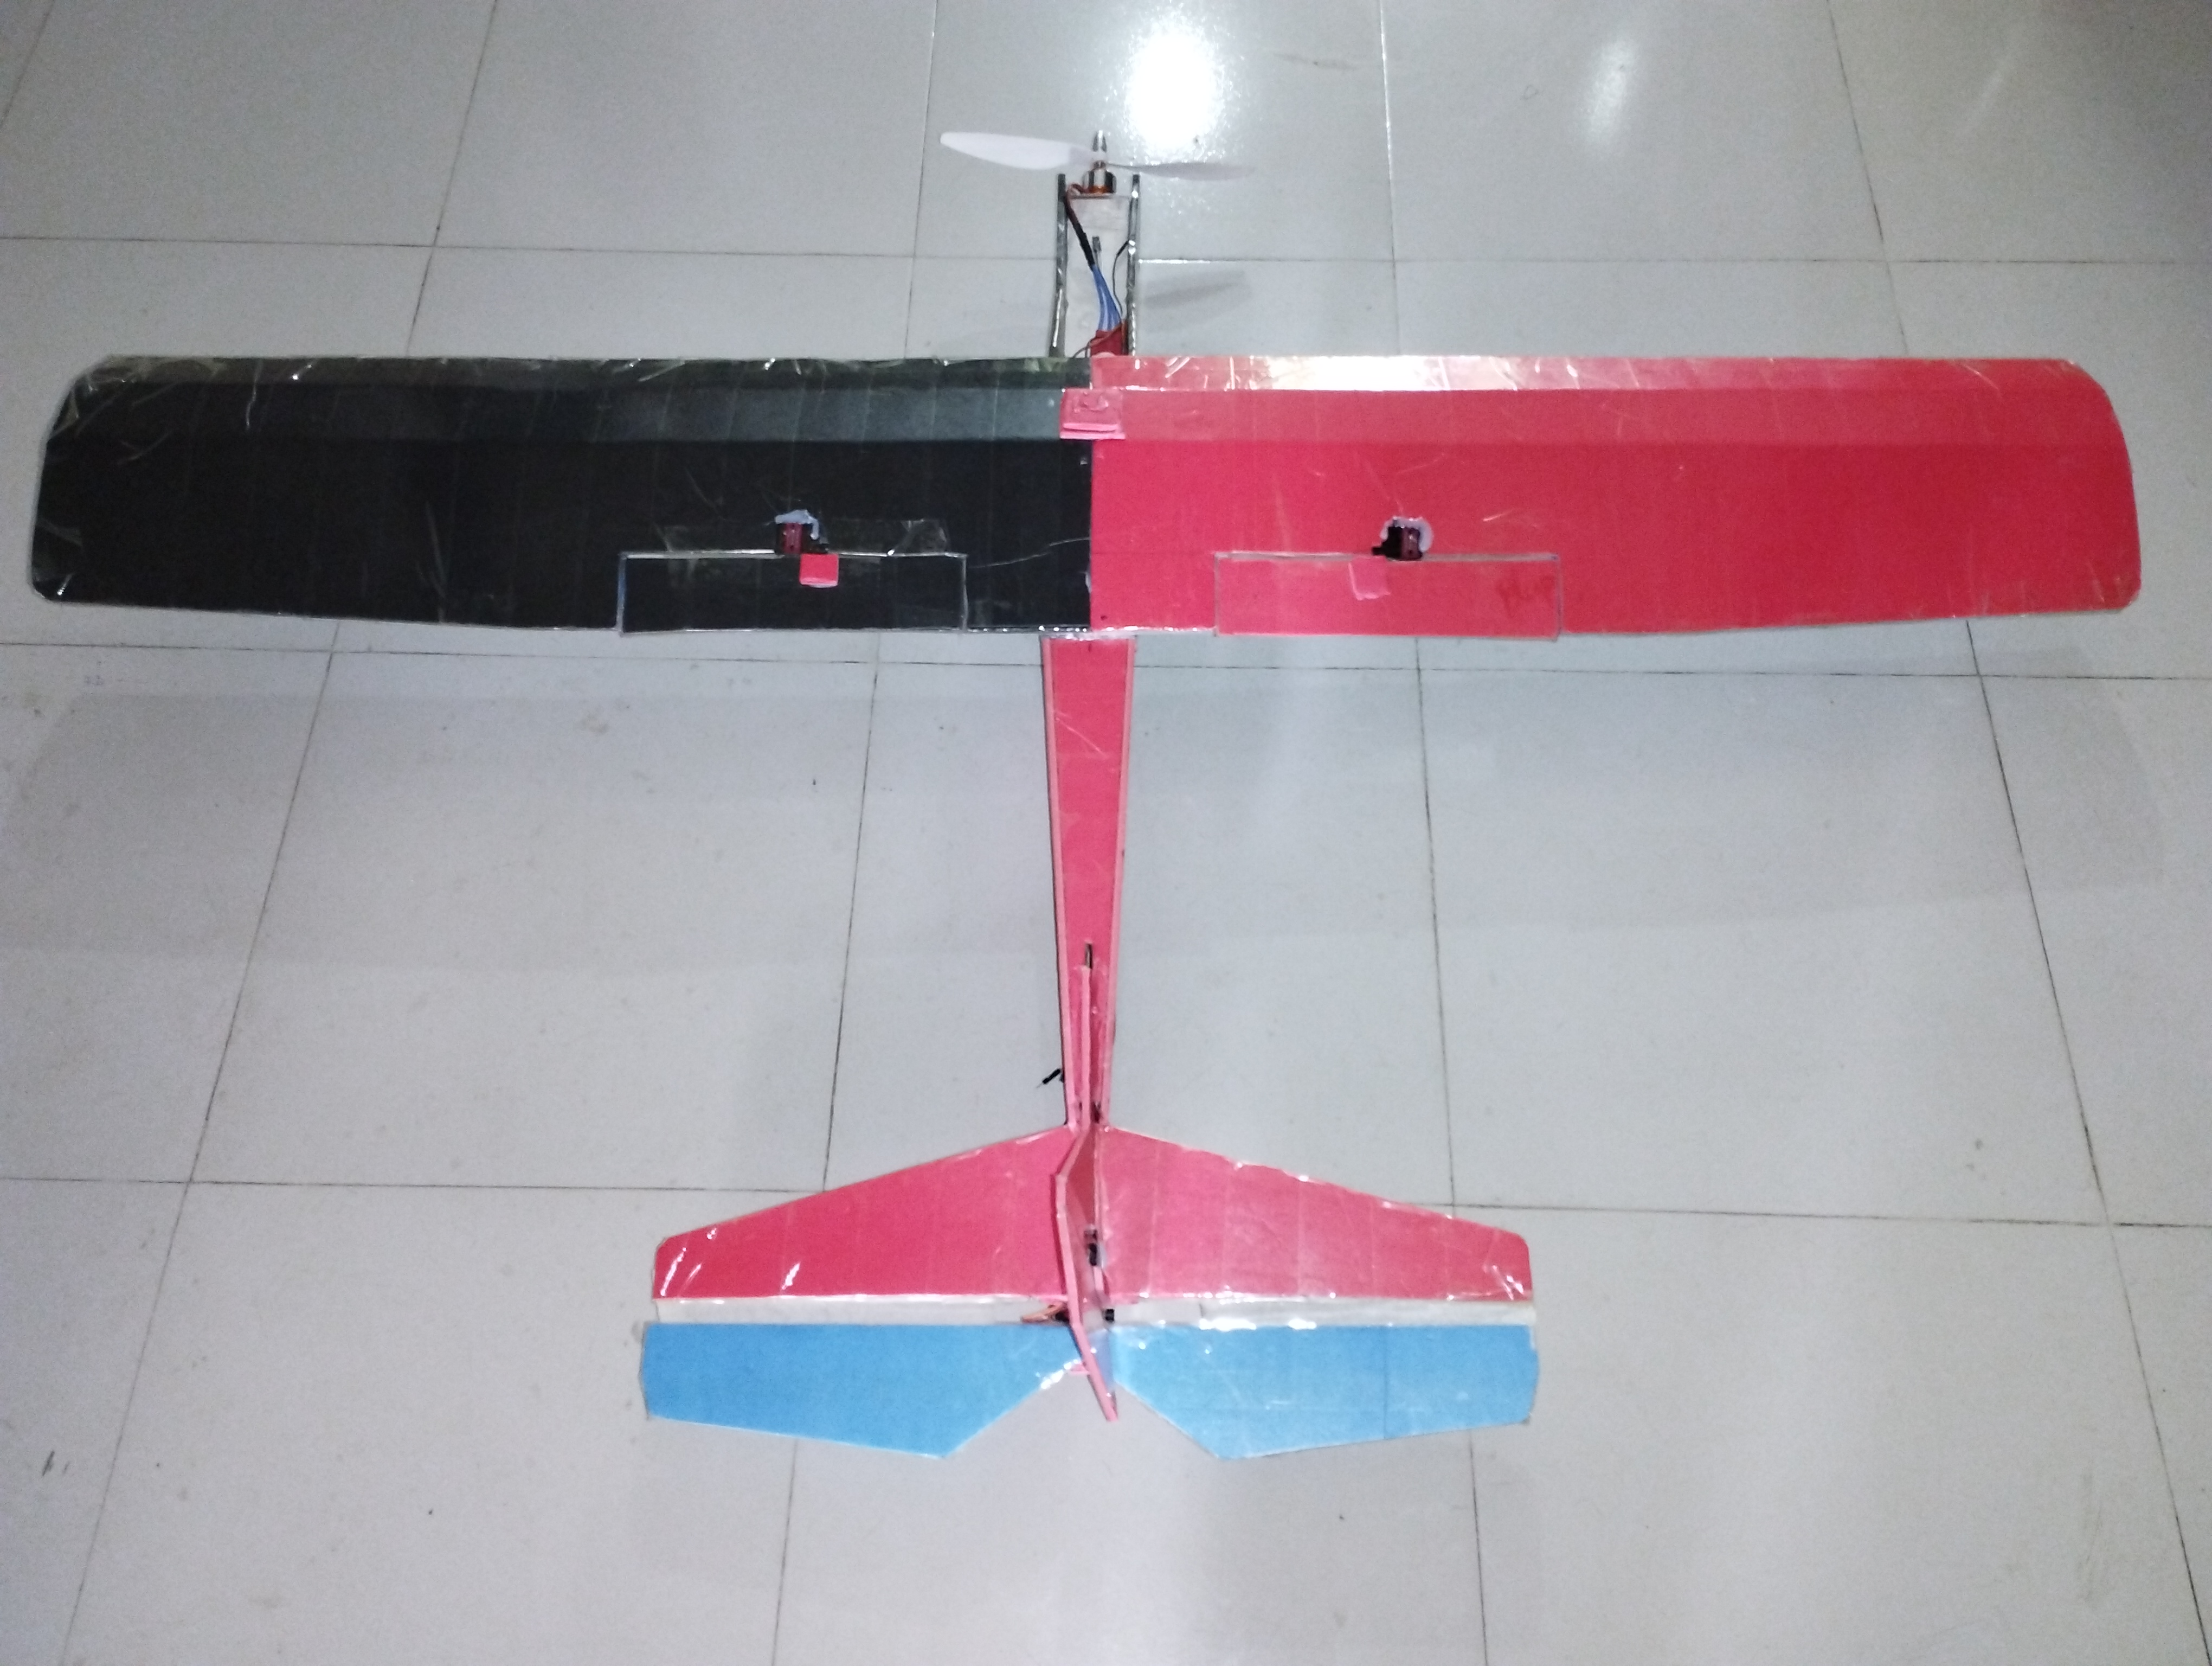
\includegraphics[width=8cm]{images/IMG_20240507_134642.jpg}
        \caption{AeroSense Explorer}
        \label{fig:enter-label}
    \end{minipage}
\end{figure}   

\begin{figure}[h]
    \begin{minipage}{0.47\textwidth}
        \flushright
        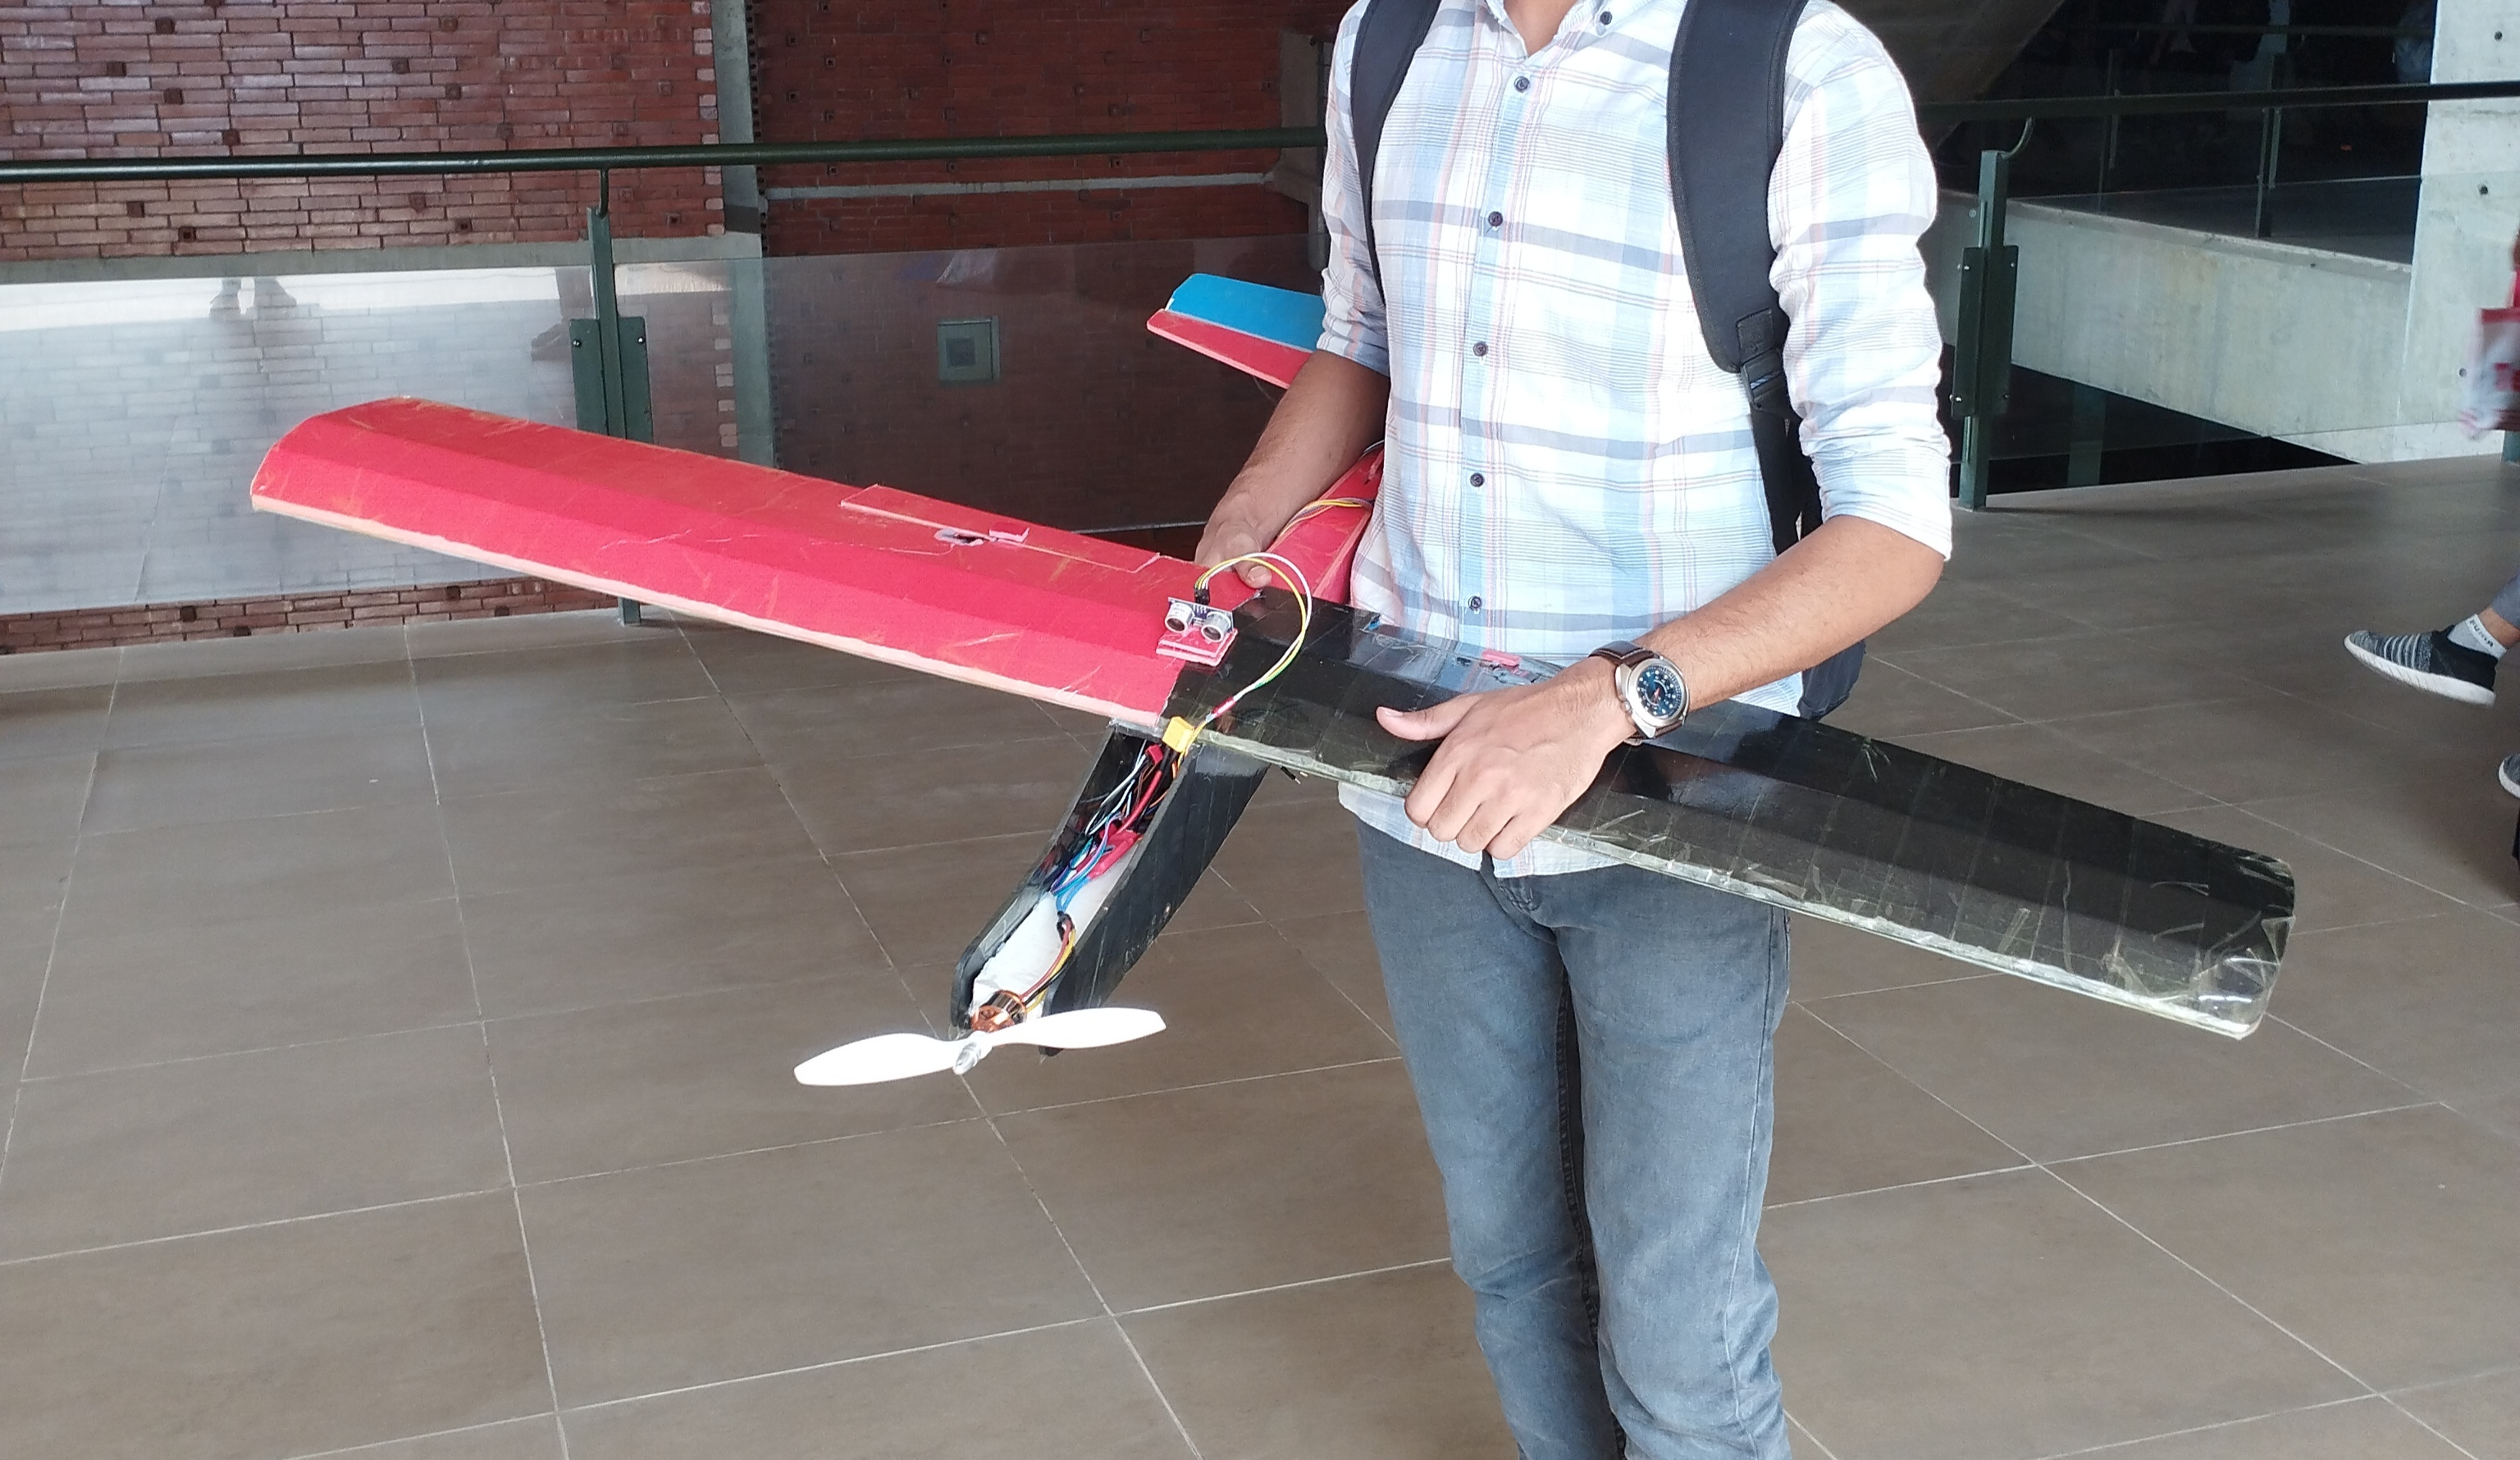
\includegraphics[width=8cm]{images/IMG_20240507_140708.jpg}
        \caption{AeroSense Explorer}
        \label{fig:enter-label}
    \end{minipage}
\end{figure}   

\begin{enumerate}

    \item Requirement Analysis: Understand the specific functionality or feature you want to implement on the fixed-wing drone. This could be anything from autonomous navigation to payload delivery.
    \item Hardware Selection: Choose the appropriate hardware components needed to support the feature. This could include flight controllers, sensors (GPS, IMU), communication modules, actuators, etc.
    \item Software Development: Develop or adapt software to control the drone and implement the desired feature. This typically involves programming the flight controller, developing algorithms for navigation or task execution, and integrating sensor data for decision-making.
    \item Testing and Debugging: Test the implemented feature in controlled environments to ensure it functions as expected. Debug any issues that arise during testing.
    \item Integration and Calibration: Integrate the software with the drone's hardware and calibrate sensors and actuators to ensure proper functionality.
    \item Field Testing: Conduct field tests to evaluate the feature's performance in real-world conditions. This may involve tweaking parameters and fine-tuning the software based on field observations.
    \item Validation and Optimization: Validate the feature against performance metrics and optimize it for better efficiency, accuracy, or reliability.
    \item Documentation and Maintenance: Document the implementation process, including software architecture, hardware setup, and operational procedures. Establish a maintenance plan to address any future updates or issues. 
\end{enumerate}
Throughout this process, safety should be a primary concern, ensuring that the implemented feature does not compromise the drone's stability or pose risks to people or property\cite{zhao2021design}.

\section{FUTURE WORK}
To achieve full autonomy in drone operation, integrating advanced technologies like GPS navigation, ground object detection, and obstacle avoidance systems is crucial. GPS navigation enables precise positioning and route planning, ensuring efficient and accurate flight paths. Ground object detection systems use sensors such as LiDAR or cameras to identify and avoid obstacles, enhancing safety during autonomous flight. Additionally, implementing machine learning algorithms can further enhance the drone's capabilities by enabling it to learn and adapt to various environments and scenarios. Through these technologies, the drone can navigate autonomously, perform tasks with minimal human intervention, and safely operate in diverse environments, opening up possibilities for applications in sectors like surveillance, agriculture, and logistics.


\section{Appendix}

\subsection{Servo and BLDC Code}

\begin{mycodelisting}{\scriptsize}

\begin{verbatim} [Servo & BLDC Code]
#include <Wire.h>
#include <Servo.h>
#include <Adafruit_PWMServoDriver.h>

Adafruit_PWMServoDriver serv
      = Adafruit_PWMServoDriver();

int th;
int yaw_l;
int yaw_r;
int pitch_up;
int pitch_down;
int roll_l;
int roll_r;

Servo th_s;

int pwm;
int ch6_lup_th = 6;
int ch4_ls_yaw = 4;
int ch2_rup_pitch = 3;
int ch1_rs_roll = 2;
int d = 0;
void setup() {
  Serial.begin(9600);
  
  serv.begin();
  serv.setPWMFreq(50);
  th_s.attach(9, 1000, 2000);
  pinMode(ch6_lup_th, INPUT);
  pinMode(ch4_ls_yaw, INPUT);
  pinMode(ch2_rup_pitch, INPUT);
  pinMode(ch1_rs_roll, INPUT);
}

void loop() {

  yaw_l = pulseIn(ch4_ls_yaw, HIGH);
  yaw_r = pulseIn(ch4_ls_yaw, HIGH);
  th = pulseIn(ch6_lup_th, HIGH);
  pitch_up = pulseIn(ch2_rup_pitch, HIGH);
  pitch_down = pulseIn(ch2_rup_pitch, HIGH);
  roll_l = pulseIn(ch1_rs_roll, HIGH);
  roll_r = pulseIn(ch1_rs_roll, HIGH);

  th = map(th, 1390, 1750, 0, 180);
  yaw_l = map(yaw_l, 2005, 1495, 89, 320);
  yaw_r = map(yaw_r, 1496, 984, 321, 551);
  pitch_up = map(pitch_up, 2005, 1495, 89, 320);
  pitch_down = map(pitch_down, 1496, 984, 321, 551);
  roll_l = map(roll_l, 2005, 1495, 89, 320);
  roll_r = map(roll_r, 1496, 984, 321, 551);
  Serial.println(pitch_up);

  th_s.write(th);
  
  serv.setPWM(1, 0, yaw_l);
  delay(d);
  
  serv.setPWM(1, 0, yaw_r);
  delay(d);
  
  serv.setPWM(2, 0, pitch_up);
  delay(d);
  
  serv.setPWM(3, 0, pitch_down);
  delay(d);
  
  serv.setPWM(4, 0, roll_l);
  delay(d);
  
  serv.setPWM(4, 0, roll_r);
  delay(d);
}
\end{verbatim} 

\end{mycodelisting}

\subsection{Sensors Code}

\begin{mycodelisting}{\scriptsize}
\begin{verbatim}[Sensors Code]
#include<SoftwareSerial.h>
SoftwareSerial B(10,11); //10-RX, 11-TX
#include <Wire.h>
#include "DHT.h"
#define DHTPIN 2
#define DHTTYPE DHT11

DHT dht(DHTPIN, DHTTYPE);

int sensorPin=A0; //mq135 pin
int sensorData;
int trigPin = 9; // TRIG pin
int echoPin = 8; // ECHO pin

float duration_us, distance_cm; 

void setup()
{  
  B.begin(9600);
  Serial.begin(9600); 
  dht.begin(); 
  pinMode(sensorPin,INPUT);        
  pinMode(trigPin, OUTPUT); 
  pinMode(echoPin, INPUT);        
            
 }
void loop()
{
  delay(2000);
  sensorData = analogRead(sensorPin);       
  Serial.print("Air Quality:");
  Serial.print(sensorData, DEC);               
  Serial.println(" PPM");
  
  digitalWrite(trigPin, HIGH);
  delayMicroseconds(10);
  digitalWrite(trigPin, LOW);
  duration_us = pulseIn(echoPin, HIGH);

  distance_cm = 0.017 * duration_us;
         
  delay(3000);

  float humi  = dht.readHumidity();
  float tempC = dht.readTemperature();
  float tempF = dht.readTemperature(true);

  if (isnan(humi) || isnan(tempC)
  || isnan(tempF)) {
    Serial.println
    ("Failed to read from DHT sensor!");
  } else {
    Serial.print("Humidity: ");
    Serial.print(humi);
    Serial.print("%");
    Serial.print("  |  "); 
    Serial.print("Temperature: ");
    Serial.print(tempC);
    Serial.print("°C ~ ");
    Serial.print(tempF);
    Serial.println("°F");
  }
  B.print(sensorData, DEC);
  B.print(" PPM");
  B.print(",");
  B.print(distance_cm);
  B.print(" CM");
  B.print(",");
  B.print(humi);
  B.print(" %");
  B.print(",");
  B.print(tempC);
  B.print(" C");
  B.print(",");
  B.print(tempF);
  B.print(" F");
  B.print(";");
  delay(20);
  }
}
\end{verbatim} 

\end{mycodelisting}

\bibliographystyle{IEEEtran}
\bibliography{sources.bib}

\begin{thebibliography}{00}

\bibitem{b1} //https://docs.arduino.cc/learn/starting-guide/whats-arduino/
https://www.makerspaces.com/arduino-uno-tutorial-beginners/
\bibitem{b2} https://components101.com/development-boards/nodemcu-esp8266-pinout-features-and-datasheet
\bibitem{b3} https://components101.com/motors/mg90s-metal-gear-servo-motor
\bibitem{b4} https://components101.com/sensors/lm35-temperature-sensor
\bibitem{b5} https://components101.com/sensors/mq135-gas-sensor-for-air-quality
\bibitem{b6} https://www.circuitbasics.com/how-to-set-up-the-dht11-humidity-sensor-on-an-arduino/
\bibitem{b7} https://components101.com/wireless/hc-06-bluetooth-module-pinout-datasheet
\bibitem{b8} https://www.rapidrcmodels.com/turnigy-d2830-11-1000kv-brushless-motor-v2-323-p.asp
\bibitem{b9} https://maker.pro/breadboard/tutorial/an-introduction-to-breadboards-and-their-uses
\bibitem{b10} https://en.wikipedia.org/wiki/Resistor

\end{thebibliography}

\end{document}

